\documentclass[landscape]{article}
\usepackage{lmodern}
\usepackage{amssymb,amsmath}
\usepackage{ifxetex,ifluatex}
\usepackage{fixltx2e} % provides \textsubscript
\ifnum 0\ifxetex 1\fi\ifluatex 1\fi=0 % if pdftex
  \usepackage[T1]{fontenc}
  \usepackage[utf8]{inputenc}
\else % if luatex or xelatex
  \ifxetex
    \usepackage{mathspec}
  \else
    \usepackage{fontspec}
  \fi
  \defaultfontfeatures{Ligatures=TeX,Scale=MatchLowercase}
\fi
% use upquote if available, for straight quotes in verbatim environments
\IfFileExists{upquote.sty}{\usepackage{upquote}}{}
% use microtype if available
\IfFileExists{microtype.sty}{%
\usepackage{microtype}
\UseMicrotypeSet[protrusion]{basicmath} % disable protrusion for tt fonts
}{}
\usepackage[margin=0.6in]{geometry}
\usepackage{hyperref}
\hypersetup{unicode=true,
            pdftitle={Chapter 12: Multicollinearity, Model Selection},
            pdfborder={0 0 0},
            breaklinks=true}
\urlstyle{same}  % don't use monospace font for urls
\usepackage{color}
\usepackage{fancyvrb}
\newcommand{\VerbBar}{|}
\newcommand{\VERB}{\Verb[commandchars=\\\{\}]}
\DefineVerbatimEnvironment{Highlighting}{Verbatim}{commandchars=\\\{\}}
% Add ',fontsize=\small' for more characters per line
\usepackage{framed}
\definecolor{shadecolor}{RGB}{248,248,248}
\newenvironment{Shaded}{\begin{snugshade}}{\end{snugshade}}
\newcommand{\KeywordTok}[1]{\textcolor[rgb]{0.13,0.29,0.53}{\textbf{#1}}}
\newcommand{\DataTypeTok}[1]{\textcolor[rgb]{0.13,0.29,0.53}{#1}}
\newcommand{\DecValTok}[1]{\textcolor[rgb]{0.00,0.00,0.81}{#1}}
\newcommand{\BaseNTok}[1]{\textcolor[rgb]{0.00,0.00,0.81}{#1}}
\newcommand{\FloatTok}[1]{\textcolor[rgb]{0.00,0.00,0.81}{#1}}
\newcommand{\ConstantTok}[1]{\textcolor[rgb]{0.00,0.00,0.00}{#1}}
\newcommand{\CharTok}[1]{\textcolor[rgb]{0.31,0.60,0.02}{#1}}
\newcommand{\SpecialCharTok}[1]{\textcolor[rgb]{0.00,0.00,0.00}{#1}}
\newcommand{\StringTok}[1]{\textcolor[rgb]{0.31,0.60,0.02}{#1}}
\newcommand{\VerbatimStringTok}[1]{\textcolor[rgb]{0.31,0.60,0.02}{#1}}
\newcommand{\SpecialStringTok}[1]{\textcolor[rgb]{0.31,0.60,0.02}{#1}}
\newcommand{\ImportTok}[1]{#1}
\newcommand{\CommentTok}[1]{\textcolor[rgb]{0.56,0.35,0.01}{\textit{#1}}}
\newcommand{\DocumentationTok}[1]{\textcolor[rgb]{0.56,0.35,0.01}{\textbf{\textit{#1}}}}
\newcommand{\AnnotationTok}[1]{\textcolor[rgb]{0.56,0.35,0.01}{\textbf{\textit{#1}}}}
\newcommand{\CommentVarTok}[1]{\textcolor[rgb]{0.56,0.35,0.01}{\textbf{\textit{#1}}}}
\newcommand{\OtherTok}[1]{\textcolor[rgb]{0.56,0.35,0.01}{#1}}
\newcommand{\FunctionTok}[1]{\textcolor[rgb]{0.00,0.00,0.00}{#1}}
\newcommand{\VariableTok}[1]{\textcolor[rgb]{0.00,0.00,0.00}{#1}}
\newcommand{\ControlFlowTok}[1]{\textcolor[rgb]{0.13,0.29,0.53}{\textbf{#1}}}
\newcommand{\OperatorTok}[1]{\textcolor[rgb]{0.81,0.36,0.00}{\textbf{#1}}}
\newcommand{\BuiltInTok}[1]{#1}
\newcommand{\ExtensionTok}[1]{#1}
\newcommand{\PreprocessorTok}[1]{\textcolor[rgb]{0.56,0.35,0.01}{\textit{#1}}}
\newcommand{\AttributeTok}[1]{\textcolor[rgb]{0.77,0.63,0.00}{#1}}
\newcommand{\RegionMarkerTok}[1]{#1}
\newcommand{\InformationTok}[1]{\textcolor[rgb]{0.56,0.35,0.01}{\textbf{\textit{#1}}}}
\newcommand{\WarningTok}[1]{\textcolor[rgb]{0.56,0.35,0.01}{\textbf{\textit{#1}}}}
\newcommand{\AlertTok}[1]{\textcolor[rgb]{0.94,0.16,0.16}{#1}}
\newcommand{\ErrorTok}[1]{\textcolor[rgb]{0.64,0.00,0.00}{\textbf{#1}}}
\newcommand{\NormalTok}[1]{#1}
\usepackage{graphicx,grffile}
\makeatletter
\def\maxwidth{\ifdim\Gin@nat@width>\linewidth\linewidth\else\Gin@nat@width\fi}
\def\maxheight{\ifdim\Gin@nat@height>\textheight\textheight\else\Gin@nat@height\fi}
\makeatother
% Scale images if necessary, so that they will not overflow the page
% margins by default, and it is still possible to overwrite the defaults
% using explicit options in \includegraphics[width, height, ...]{}
\setkeys{Gin}{width=\maxwidth,height=\maxheight,keepaspectratio}
\IfFileExists{parskip.sty}{%
\usepackage{parskip}
}{% else
\setlength{\parindent}{0pt}
\setlength{\parskip}{6pt plus 2pt minus 1pt}
}
\setlength{\emergencystretch}{3em}  % prevent overfull lines
\providecommand{\tightlist}{%
  \setlength{\itemsep}{0pt}\setlength{\parskip}{0pt}}
\setcounter{secnumdepth}{0}
% Redefines (sub)paragraphs to behave more like sections
\ifx\paragraph\undefined\else
\let\oldparagraph\paragraph
\renewcommand{\paragraph}[1]{\oldparagraph{#1}\mbox{}}
\fi
\ifx\subparagraph\undefined\else
\let\oldsubparagraph\subparagraph
\renewcommand{\subparagraph}[1]{\oldsubparagraph{#1}\mbox{}}
\fi

%%% Use protect on footnotes to avoid problems with footnotes in titles
\let\rmarkdownfootnote\footnote%
\def\footnote{\protect\rmarkdownfootnote}

%%% Change title format to be more compact
\usepackage{titling}

% Create subtitle command for use in maketitle
\newcommand{\subtitle}[1]{
  \posttitle{
    \begin{center}\large#1\end{center}
    }
}

\setlength{\droptitle}{-2em}

  \title{Chapter 12: Multicollinearity, Model Selection}
    \pretitle{\vspace{\droptitle}\centering\huge}
  \posttitle{\par}
    \author{}
    \preauthor{}\postauthor{}
    \date{}
    \predate{}\postdate{}
  
\usepackage{soul}
\usepackage{booktabs}

\begin{document}
\maketitle

\subsection{Context}\label{context}

\paragraph{Intro to data}\label{intro-to-data}

Our data set comes from Ericksen et al. (1989), who were expert
witnesses in a US Supreme Court case about corrections to the U.S.
Census undercount. (The descriptive text here quotes from that article.)
This is important because Census numbers are used in many ways
throughout the government, including setting the amount of funding that
is passed from the federal government to those locations. Several cities
and states sued the U.S. Census Bureau, to correct the census results.
One of the arguments made was that census undercounts were primarily
concentrated in regions with high prevalence of minorities.

We have measurements on 66 different regions in the U.S.: 16 large
cities, the remaining parts of the states in which these cities are
located, and the other U.S. states. For each of these regions, we have:

\begin{itemize}
\tightlist
\item
  \texttt{name}: The name of the region.
\item
  \texttt{minority}: Percentage black or Hispanic.
\item
  \texttt{crime}: Rate of serious crimes per 1000 population.
\item
  \texttt{poverty}: Percentage poor.
\item
  \texttt{language}: Percentage having difficulty speaking or writing
  English.
\item
  \texttt{highschool}: Percentage age 25 or older who had not finished
  highschool.
\item
  \texttt{housing}: Percentage of housing in small, multiunit buildings.
\item
  \texttt{geographic\_unit}: ``city'' or ``state''.
\item
  \texttt{conventional}: Percentage of households counted by
  conventional personal enumeration (the method in primary use up until
  about 1950, and used less in 1980).
\item
  \texttt{undercount}: Preliminary estimate of percentage undercount,
  based on a second survey.
\end{itemize}

\begin{Shaded}
\begin{Highlighting}[]
\KeywordTok{head}\NormalTok{(census, }\DecValTok{3}\NormalTok{)}
\end{Highlighting}
\end{Shaded}

\begin{verbatim}
##      name minority crime poverty language highschool housing geographic_unit conventional undercount
## 1 Alabama     26.1    49    18.9      0.2       43.5     7.6           state            0      -0.04
## 2  Alaska      5.7    62    10.7      1.7       17.5    23.6           state          100       3.35
## 3 Arizona     18.9    81    13.2      3.2       27.6     8.1           state           18       2.48
\end{verbatim}

References:

\begin{itemize}
\tightlist
\item
  Fox, J. and Weisberg, S. (2011) An R Companion to Applied Regression,
  Second Edition, Sage.
\item
  Ericksen, E. P., Kadane, J. B. and Tukey, J. W. (1989) Adjusting the
  1980 Census of Population and Housing. \emph{Journal of the American
  Statistical Association} 84, 927--944.
\end{itemize}

Let's consider a model for \texttt{undercount} (response) based on all
of the other explanatory variables in the data set (other than the name
of the location).

\paragraph{Pairs Plots}\label{pairs-plots}

\begin{Shaded}
\begin{Highlighting}[]
\KeywordTok{library}\NormalTok{(GGally)}
\KeywordTok{ggpairs}\NormalTok{(census }\OperatorTok\StringTok{ }\KeywordTok{select}\NormalTok{(}\OperatorTok{-}\NormalTok{name))}
\end{Highlighting}
\end{Shaded}

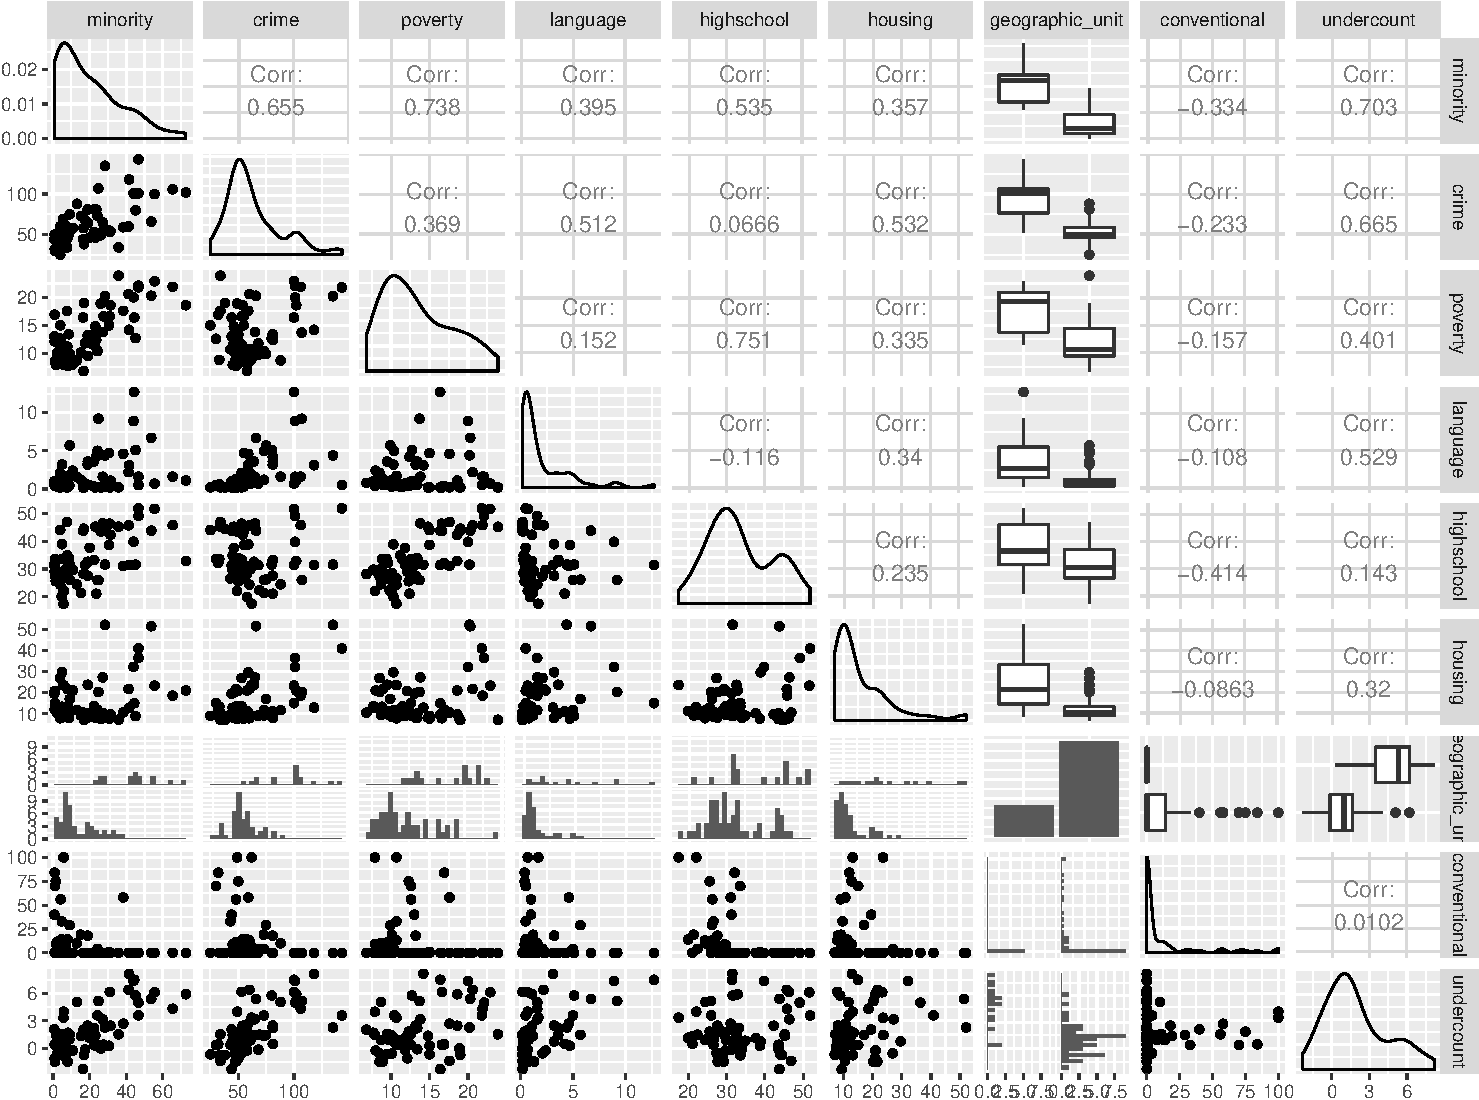
\includegraphics{20190422_multicollinearity_files/figure-latex/unnamed-chunk-2-1.pdf}

\newpage

\begin{Shaded}
\begin{Highlighting}[]
\NormalTok{census_transformed <-}\StringTok{ }\NormalTok{census }\OperatorTok
\StringTok{  }\KeywordTok{transmute}\NormalTok{(}
    \DataTypeTok{minority =}\NormalTok{ minority}\OperatorTok{^}\FloatTok{0.75}\NormalTok{,}
    \DataTypeTok{crime =} \KeywordTok{log}\NormalTok{(crime),}
    \DataTypeTok{poverty =} \KeywordTok{sqrt}\NormalTok{(poverty),}
    \DataTypeTok{language =} \KeywordTok{sqrt}\NormalTok{(language),}
    \DataTypeTok{highschool =}\NormalTok{ highschool,}
    \DataTypeTok{housing =} \KeywordTok{log}\NormalTok{(housing),}
    \DataTypeTok{geographic_unit =}\NormalTok{ geographic_unit,}
    \DataTypeTok{conventional =} \KeywordTok{log}\NormalTok{(conventional }\OperatorTok{+}\StringTok{ }\DecValTok{1}\NormalTok{),}
    \DataTypeTok{undercount =}\NormalTok{ undercount}
\NormalTok{  )}
\end{Highlighting}
\end{Shaded}

\begin{Shaded}
\begin{Highlighting}[]
\KeywordTok{ggpairs}\NormalTok{(census_transformed)}
\end{Highlighting}
\end{Shaded}

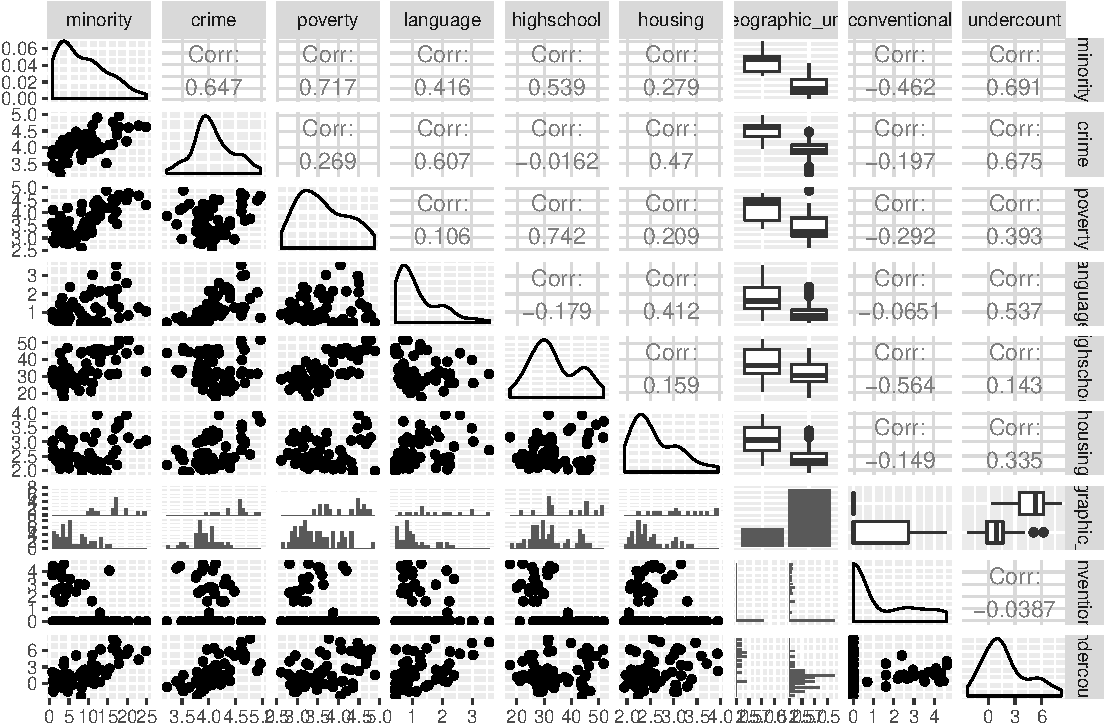
\includegraphics{20190422_multicollinearity_files/figure-latex/unnamed-chunk-4-1.pdf}

\newpage

\subsection{Challenge:
Multicollinearity}\label{challenge-multicollinearity}

\begin{itemize}
\tightlist
\item
  \textbf{Multicollinearity:} Some of the explanatory variables are
  linearly associated with each other. Effects:

  \begin{itemize}
  \tightlist
  \item
    Apparent association between a given explanatory variable and the
    response can change if we add or remove other explanatory variables
    from the model.
  \item
    Standard errors of coefficient estimates are large.

    \begin{itemize}
    \tightlist
    \item
      We are not certain of the coefficient value: which of the
      correlated explanatory variables is actually responsible for
      changes in the response?
    \item
      This can lead to small t statistics/large p-values even if a
      variable is associated with the response.
    \end{itemize}
  \end{itemize}
\end{itemize}

\paragraph{Illustration, focusing on just the crime and housing
explanatory
variables}\label{illustration-focusing-on-just-the-crime-and-housing-explanatory-variables}

\begin{Shaded}
\begin{Highlighting}[]
\KeywordTok{ggpairs}\NormalTok{(census_transformed }\OperatorTok\StringTok{ }\KeywordTok{select}\NormalTok{(crime, housing, undercount))}
\end{Highlighting}
\end{Shaded}

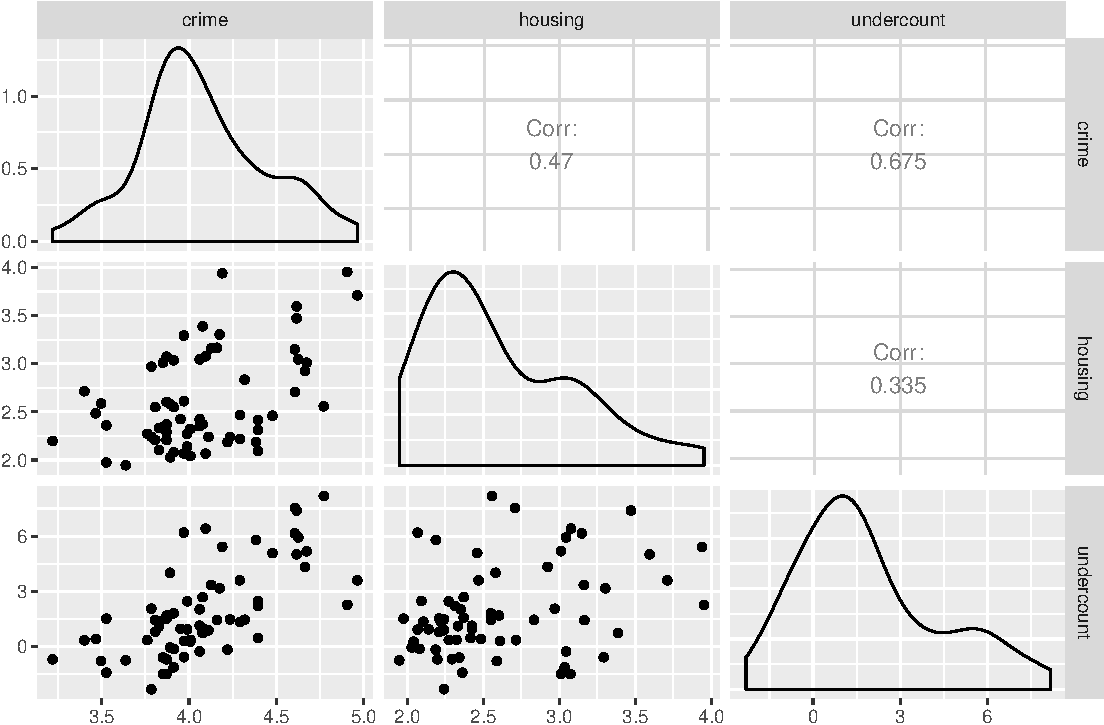
\includegraphics{20190422_multicollinearity_files/figure-latex/unnamed-chunk-5-1.pdf}

\newpage

\begin{Shaded}
\begin{Highlighting}[]
\NormalTok{lm_highschool <-}\StringTok{ }\KeywordTok{lm}\NormalTok{(undercount }\OperatorTok{~}\StringTok{ }\NormalTok{crime, }\DataTypeTok{data =}\NormalTok{ census_transformed)}
\KeywordTok{summary}\NormalTok{(lm_highschool)}
\end{Highlighting}
\end{Shaded}

\begin{verbatim}
## 
## Call:
## lm(formula = undercount ~ crime, data = census_transformed)
## 
## Residuals:
##     Min      1Q  Median      3Q     Max 
## -3.4388 -1.2250 -0.0878  1.1312  4.7525 
## 
## Coefficients:
##             Estimate Std. Error t value Pr(>|t|)    
## (Intercept) -16.6997     2.5562  -6.533 1.22e-08 ***
## crime         4.5682     0.6246   7.313 5.23e-10 ***
## ---
## Signif. codes:  0 '***' 0.001 '**' 0.01 '*' 0.05 '.' 0.1 ' ' 1
## 
## Residual standard error: 1.838 on 64 degrees of freedom
## Multiple R-squared:  0.4553, Adjusted R-squared:  0.4467 
## F-statistic: 53.49 on 1 and 64 DF,  p-value: 5.233e-10
\end{verbatim}

\begin{Shaded}
\begin{Highlighting}[]
\NormalTok{lm_poverty <-}\StringTok{ }\KeywordTok{lm}\NormalTok{(undercount }\OperatorTok{~}\StringTok{ }\NormalTok{housing, }\DataTypeTok{data =}\NormalTok{ census_transformed)}
\KeywordTok{summary}\NormalTok{(lm_poverty)}
\end{Highlighting}
\end{Shaded}

\begin{verbatim}
## 
## Call:
## lm(formula = undercount ~ housing, data = census_transformed)
## 
## Residuals:
##     Min      1Q  Median      3Q     Max 
## -4.1672 -1.3946 -0.2819  1.1527  6.3489 
## 
## Coefficients:
##             Estimate Std. Error t value Pr(>|t|)   
## (Intercept)  -2.4163     1.5506  -1.558  0.12409   
## housing       1.6609     0.5834   2.847  0.00592 **
## ---
## Signif. codes:  0 '***' 0.001 '**' 0.01 '*' 0.05 '.' 0.1 ' ' 1
## 
## Residual standard error: 2.346 on 64 degrees of freedom
## Multiple R-squared:  0.1124, Adjusted R-squared:  0.09854 
## F-statistic: 8.106 on 1 and 64 DF,  p-value: 0.005925
\end{verbatim}

\begin{Shaded}
\begin{Highlighting}[]
\NormalTok{lm_highschool_poverty <-}\StringTok{ }\KeywordTok{lm}\NormalTok{(undercount }\OperatorTok{~}\StringTok{ }\NormalTok{crime }\OperatorTok{+}\StringTok{ }\NormalTok{housing, }\DataTypeTok{data =}\NormalTok{ census_transformed)}
\KeywordTok{summary}\NormalTok{(lm_highschool_poverty)}
\end{Highlighting}
\end{Shaded}

\begin{verbatim}
## 
## Call:
## lm(formula = undercount ~ crime + housing, data = census_transformed)
## 
## Residuals:
##     Min      1Q  Median      3Q     Max 
## -3.5308 -1.2343 -0.0999  1.0951  4.8067 
## 
## Coefficients:
##             Estimate Std. Error t value Pr(>|t|)    
## (Intercept) -16.6986     2.5754  -6.484 1.57e-08 ***
## crime         4.4950     0.7132   6.303 3.22e-08 ***
## housing       0.1139     0.5218   0.218    0.828    
## ---
## Signif. codes:  0 '***' 0.001 '**' 0.01 '*' 0.05 '.' 0.1 ' ' 1
## 
## Residual standard error: 1.852 on 63 degrees of freedom
## Multiple R-squared:  0.4557, Adjusted R-squared:  0.4384 
## F-statistic: 26.37 on 2 and 63 DF,  p-value: 4.785e-09
\end{verbatim}

\newpage

\begin{Shaded}
\begin{Highlighting}[]
\NormalTok{p1 <-}\StringTok{ }\KeywordTok{ggplot}\NormalTok{(}\DataTypeTok{data =}\NormalTok{ census_transformed, }\DataTypeTok{mapping =} \KeywordTok{aes}\NormalTok{(}\DataTypeTok{x =}\NormalTok{ crime, }\DataTypeTok{y =}\NormalTok{ undercount)) }\OperatorTok{+}
\StringTok{  }\KeywordTok{geom_point}\NormalTok{() }\OperatorTok{+}
\StringTok{  }\KeywordTok{geom_smooth}\NormalTok{(}\DataTypeTok{method =} \StringTok{"lm"}\NormalTok{, }\DataTypeTok{se =} \OtherTok{FALSE}\NormalTok{) }\OperatorTok{+}
\StringTok{  }\KeywordTok{theme_bw}\NormalTok{()}

\NormalTok{p2 <-}\StringTok{ }\KeywordTok{ggplot}\NormalTok{(}\DataTypeTok{data =}\NormalTok{ census_transformed, }\DataTypeTok{mapping =} \KeywordTok{aes}\NormalTok{(}\DataTypeTok{x =}\NormalTok{ housing, }\DataTypeTok{y =}\NormalTok{ undercount)) }\OperatorTok{+}
\StringTok{  }\KeywordTok{geom_point}\NormalTok{() }\OperatorTok{+}
\StringTok{  }\KeywordTok{geom_smooth}\NormalTok{(}\DataTypeTok{method =} \StringTok{"lm"}\NormalTok{, }\DataTypeTok{se =} \OtherTok{FALSE}\NormalTok{) }\OperatorTok{+}
\StringTok{  }\KeywordTok{theme_bw}\NormalTok{()}

\KeywordTok{grid.arrange}\NormalTok{(p1, p2, }\DataTypeTok{ncol =} \DecValTok{2}\NormalTok{)}
\end{Highlighting}
\end{Shaded}

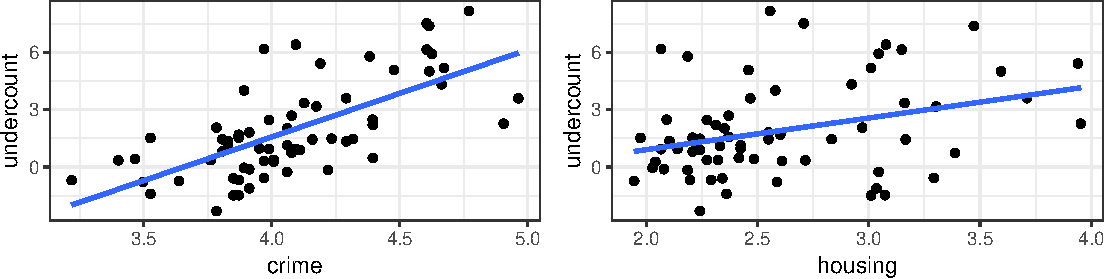
\includegraphics{20190422_multicollinearity_files/figure-latex/unnamed-chunk-7-1.pdf}

\begin{Shaded}
\begin{Highlighting}[]
\KeywordTok{library}\NormalTok{(car)}
\KeywordTok{avPlots}\NormalTok{(lm_highschool_poverty)}
\end{Highlighting}
\end{Shaded}

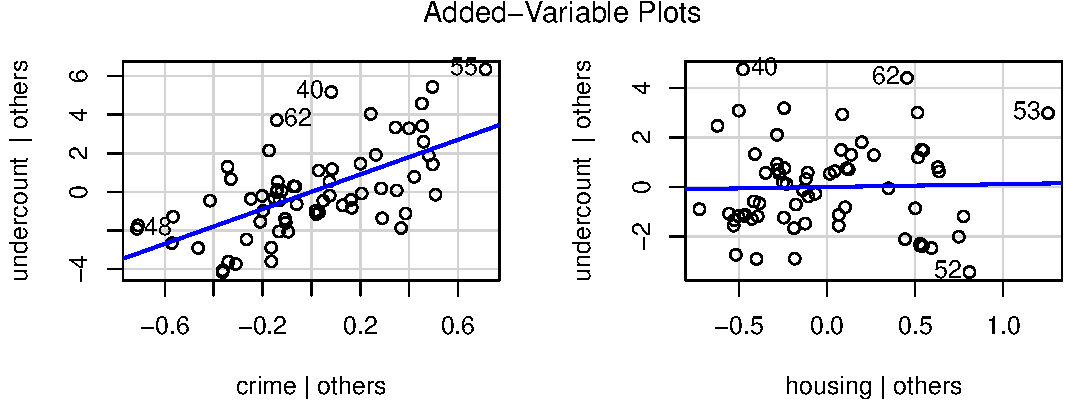
\includegraphics{20190422_multicollinearity_files/figure-latex/unnamed-chunk-8-1.pdf}

\newpage

\subsection{A model with all the explanatory
variables}\label{a-model-with-all-the-explanatory-variables}

\begin{Shaded}
\begin{Highlighting}[]
\NormalTok{bigfit <-}\StringTok{ }\KeywordTok{lm}\NormalTok{(undercount }\OperatorTok{~}\StringTok{ }\NormalTok{minority }\OperatorTok{+}\StringTok{ }\NormalTok{crime }\OperatorTok{+}\StringTok{ }\NormalTok{poverty }\OperatorTok{+}\StringTok{ }\NormalTok{language }\OperatorTok{+}\StringTok{ }\NormalTok{highschool }\OperatorTok{+}\StringTok{ }\NormalTok{housing }\OperatorTok{+}\StringTok{ }\NormalTok{geographic_unit }\OperatorTok{+}\StringTok{ }\NormalTok{conventional,}
    \DataTypeTok{data =}\NormalTok{ census_transformed)}
\KeywordTok{summary}\NormalTok{(bigfit)}
\end{Highlighting}
\end{Shaded}

\begin{verbatim}
## 
## Call:
## lm(formula = undercount ~ minority + crime + poverty + language + 
##     highschool + housing + geographic_unit + conventional, data = census_transformed)
## 
## Residuals:
##     Min      1Q  Median      3Q     Max 
## -2.8986 -0.9230  0.1316  0.7453  4.4242 
## 
## Coefficients:
##                      Estimate Std. Error t value Pr(>|t|)    
## (Intercept)          -2.64397    4.40182  -0.601 0.550451    
## minority              0.21050    0.07229   2.912 0.005118 ** 
## crime                 1.38213    0.92024   1.502 0.138636    
## poverty              -1.13818    0.62294  -1.827 0.072922 .  
## language              0.58031    0.35387   1.640 0.106538    
## highschool            0.07221    0.04925   1.466 0.148128    
## housing              -0.42226    0.51322  -0.823 0.414070    
## geographic_unitstate -1.93606    0.79686  -2.430 0.018289 *  
## conventional          0.66436    0.16203   4.100 0.000132 ***
## ---
## Signif. codes:  0 '***' 0.001 '**' 0.01 '*' 0.05 '.' 0.1 ' ' 1
## 
## Residual standard error: 1.449 on 57 degrees of freedom
## Multiple R-squared:  0.6982, Adjusted R-squared:  0.6559 
## F-statistic: 16.48 on 8 and 57 DF,  p-value: 2.495e-12
\end{verbatim}

It seems like we probably don't need all of those variables in the
model.

\newpage

\paragraph{Variance Inflation Factors}\label{variance-inflation-factors}

\begin{itemize}
\tightlist
\item
  ``How much larger is the variance of \(\hat{\beta}_j\) than it would
  be if all explanatory variables were uncorrelated?''
\end{itemize}

\begin{Shaded}
\begin{Highlighting}[]
\KeywordTok{vif}\NormalTok{(bigfit)}
\end{Highlighting}
\end{Shaded}

\begin{verbatim}
##        minority           crime         poverty        language      highschool         housing geographic_unit    conventional 
##        6.067582        3.489176        4.273742        2.037437        5.414260        2.027117        3.663772        2.068474
\end{verbatim}

\begin{itemize}
\tightlist
\item
  A VIF of \(4\) means our confidence interval for that coefficient is
  twice as wide as it would be if all explanatory variables were
  uncorrelated.
\end{itemize}

\vspace{3cm}

\begin{itemize}
\tightlist
\item
  As a rough guide, a VIF \(> 5\) indicates we may want to do something
  to address multicollinearity.

  \begin{itemize}
  \tightlist
  \item
    In this class, that means drop explanatory variables that don't help
    the model but do inflate variances
  \item
    Other strategies include principle components analysis and penalized
    regression; see stat 340/other classes!
  \end{itemize}
\item
  \(VIF = \frac{1}{1 - R_X^2}\), where \(R_X^2\) is the \(R^2\) of the
  regression of the given explanatory variable on all other explanatory
  variables.
\end{itemize}

\subsection{Which explanatory variables should we include in our
model?}\label{which-explanatory-variables-should-we-include-in-our-model}

Note: this topic will be explored in much more depth in Statistics 340.
We introduce some first ideas here.

\paragraph{Basic Motivations}\label{basic-motivations}

\begin{itemize}
\tightlist
\item
  Need \textbf{enough}:

  \begin{itemize}
  \tightlist
  \item
    Include all the important variables we are interested in/necessary
    to answer our scientific questions
  \item
    Include any important potential confounding variables
  \end{itemize}
\item
  But \textbf{not too many}:

  \begin{itemize}
  \tightlist
  \item
    Try to avoid including highly correlated explanatory variables,
    unless we really need them.
  \end{itemize}
\item
  Acknowledge \textbf{there is no perfect model}:

  \begin{itemize}
  \tightlist
  \item
    We will probably identify multiple sets of explanatory variables
    that are about as good as each other.
  \item
    We should present results from all of these models (or a
    representative group of them).
  \end{itemize}
\item
  Our goal is \textbf{not} to find models that support our favorite
  theories/get us statistically significant results/etc.!
\item
  \textbf{Our goal is to see what the data can and can not tell us about
  what we're studying}
\end{itemize}

\newpage

\paragraph{All Subsets Regression}\label{all-subsets-regression}

\begin{itemize}
\tightlist
\item
  Fit every possible model based on all the different subsets of
  explanatory variables

  \begin{itemize}
  \tightlist
  \item
    Model with only minority
  \item
    \ldots{}all other models with one explanatory variable\ldots{}
  \item
    Model with minority and crime
  \item
    \ldots{}all other models with 2, 3, 4, 5, 6, or 7 explanatory
    variables\ldots{}
  \item
    Model with all 8 explanatory variables
  \end{itemize}
\item
  Pick ``best'' models to discuss
\end{itemize}

\begin{Shaded}
\begin{Highlighting}[]
\KeywordTok{library}\NormalTok{(leaps)}
\NormalTok{candidate_models <-}\StringTok{ }\KeywordTok{regsubsets}\NormalTok{(}
\NormalTok{  undercount }\OperatorTok{~}\StringTok{ }\NormalTok{minority }\OperatorTok{+}\StringTok{ }\NormalTok{crime }\OperatorTok{+}\StringTok{ }\NormalTok{poverty }\OperatorTok{+}\StringTok{ }\NormalTok{language }\OperatorTok{+}\StringTok{ }\NormalTok{highschool }\OperatorTok{+}\StringTok{ }\NormalTok{housing }\OperatorTok{+}\StringTok{ }\NormalTok{geographic_unit }\OperatorTok{+}\StringTok{ }\NormalTok{conventional,}
  \DataTypeTok{data =}\NormalTok{ census_transformed,}
  \DataTypeTok{nbest =} \DecValTok{1}\NormalTok{)}
\KeywordTok{summary}\NormalTok{(candidate_models)}
\end{Highlighting}
\end{Shaded}

\begin{verbatim}
## Subset selection object
## Call: regsubsets.formula(undercount ~ minority + crime + poverty + 
##     language + highschool + housing + geographic_unit + conventional, 
##     data = census_transformed, nbest = 1)
## 8 Variables  (and intercept)
##                      Forced in Forced out
## minority                 FALSE      FALSE
## crime                    FALSE      FALSE
## poverty                  FALSE      FALSE
## language                 FALSE      FALSE
## highschool               FALSE      FALSE
## housing                  FALSE      FALSE
## geographic_unitstate     FALSE      FALSE
## conventional             FALSE      FALSE
## 1 subsets of each size up to 8
## Selection Algorithm: exhaustive
##          minority crime poverty language highschool housing geographic_unitstate conventional
## 1  ( 1 ) "*"      " "   " "     " "      " "        " "     " "                  " "         
## 2  ( 1 ) "*"      " "   " "     " "      " "        " "     " "                  "*"         
## 3  ( 1 ) "*"      "*"   " "     " "      " "        " "     " "                  "*"         
## 4  ( 1 ) "*"      " "   "*"     " "      " "        " "     "*"                  "*"         
## 5  ( 1 ) "*"      " "   "*"     "*"      " "        " "     "*"                  "*"         
## 6  ( 1 ) "*"      "*"   "*"     "*"      " "        " "     "*"                  "*"         
## 7  ( 1 ) "*"      "*"   "*"     "*"      "*"        " "     "*"                  "*"         
## 8  ( 1 ) "*"      "*"   "*"     "*"      "*"        "*"     "*"                  "*"
\end{verbatim}

\begin{itemize}
\tightlist
\item
  For a particular number of explanatory variables, ``best'' models have
  smallest sum of squared residuals
\item
  How should we select the number of explanatory variables to use?
\end{itemize}

\newpage

\paragraph{\texorpdfstring{\emph{Not} by looking for smallest sum of
squared
residuals}{Not by looking for smallest sum of squared residuals}}\label{not-by-looking-for-smallest-sum-of-squared-residuals}

\begin{itemize}
\tightlist
\item
  Adding more explanatory variables will \emph{always} reduce sum of
  squared residuals, but may not give a better model
\end{itemize}

\begin{Shaded}
\begin{Highlighting}[]
\KeywordTok{summary}\NormalTok{(candidate_models)}\OperatorTok{$}\NormalTok{rss}
\end{Highlighting}
\end{Shaded}

\begin{verbatim}
## [1] 207.5440 167.7937 142.1790 131.3334 126.4677 124.4305 121.1672 119.7451
\end{verbatim}

\paragraph{\texorpdfstring{\emph{Not} by looking for largest
\(R^2\)}{Not by looking for largest R\^{}2}}\label{not-by-looking-for-largest-r2}

\begin{itemize}
\tightlist
\item
  Adding more explanatory variables will \emph{always} increase \(R^2\),
  but may not give a better model
\end{itemize}

\begin{Shaded}
\begin{Highlighting}[]
\KeywordTok{summary}\NormalTok{(candidate_models)}\OperatorTok{$}\NormalTok{rsq}
\end{Highlighting}
\end{Shaded}

\begin{verbatim}
## [1] 0.4769295 0.5771118 0.6416680 0.6690021 0.6812651 0.6863994 0.6946239 0.6982080
\end{verbatim}

\paragraph{One Option: BIC}\label{one-option-bic}

\begin{itemize}
\tightlist
\item
  We want a criterion that says ``Make the Residual Sum of Squares
  small, but don't include too many explanatory variables''
\item
  Bayesian Information Criterion: Minimize
  \[BIC = n \times \log\left( \frac{\text{Sum of Squared Residuals}}{n} \right) + \log(n) \times (p + 1)\]
\item
  The first term is small if the Sum of Squared Residuals is small
\item
  The second term is small if the number of explanatory variables,
  \(p\), is small
\end{itemize}

\begin{Shaded}
\begin{Highlighting}[]
\KeywordTok{summary}\NormalTok{(candidate_models)}\OperatorTok{$}\NormalTok{bic}
\end{Highlighting}
\end{Shaded}

\begin{verbatim}
## [1] -34.39127 -44.23377 -50.97688 -52.02418 -50.32618 -47.20833 -44.77270 -41.36226
\end{verbatim}

\begin{Shaded}
\begin{Highlighting}[]
\KeywordTok{plot}\NormalTok{(candidate_models)}
\end{Highlighting}
\end{Shaded}

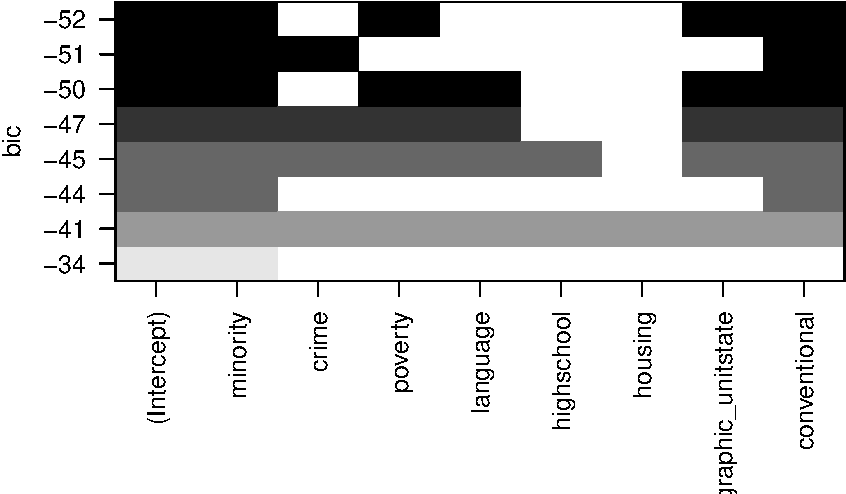
\includegraphics{20190422_multicollinearity_files/figure-latex/unnamed-chunk-15-1.pdf}

\begin{itemize}
\tightlist
\item
  Generally, models with BIC within about 2 of the smallest BIC are
  equivalent in terms of utility.

  \begin{itemize}
  \tightlist
  \item
    We should report on \textbf{all 3} of the models with lowest BIC
    here.
  \end{itemize}
\item
  We could also look at more than 1 ``best model'' of each size
\end{itemize}

\begin{Shaded}
\begin{Highlighting}[]
\NormalTok{candidate_models3 <-}\StringTok{ }\KeywordTok{regsubsets}\NormalTok{(}
\NormalTok{  undercount }\OperatorTok{~}\StringTok{ }\NormalTok{minority }\OperatorTok{+}\StringTok{ }\NormalTok{crime }\OperatorTok{+}\StringTok{ }\NormalTok{poverty }\OperatorTok{+}\StringTok{ }\NormalTok{language }\OperatorTok{+}\StringTok{ }\NormalTok{highschool }\OperatorTok{+}\StringTok{ }\NormalTok{housing }\OperatorTok{+}\StringTok{ }\NormalTok{geographic_unit }\OperatorTok{+}\StringTok{ }\NormalTok{conventional,}
  \DataTypeTok{data =}\NormalTok{ census_transformed,}
  \DataTypeTok{nbest =} \DecValTok{3}\NormalTok{)}
\KeywordTok{plot}\NormalTok{(candidate_models3)}
\end{Highlighting}
\end{Shaded}

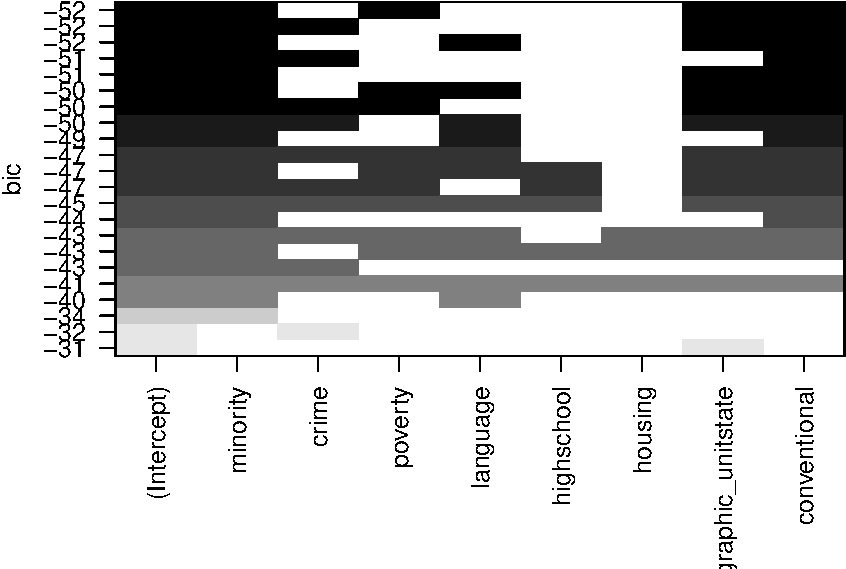
\includegraphics{20190422_multicollinearity_files/figure-latex/unnamed-chunk-16-1.pdf}

\begin{Shaded}
\begin{Highlighting}[]
\KeywordTok{summary}\NormalTok{(candidate_models3)}\OperatorTok{$}\NormalTok{bic }\OperatorTok
\StringTok{  }\KeywordTok{sort}\NormalTok{()}
\end{Highlighting}
\end{Shaded}

\begin{verbatim}
##  [1] -52.02418 -51.76637 -51.55289 -50.97688 -50.84480 -50.32618 -49.96010 -49.70790 -48.66521 -47.20833 -47.02759 -46.56884 -44.77270 -44.23377 -43.10900
## [16] -42.99031 -42.55693 -41.36226 -40.48006 -34.39127 -31.71105 -30.78063
\end{verbatim}

\begin{itemize}
\tightlist
\item
  In an actual analysis, I would examine and report on \textbf{all 6} of
  the models with lowest BIC. (Not doing that here for the sake of
  time/space/our attention spans.)
\end{itemize}

\newpage

\subsection{Finishing off the
analysis}\label{finishing-off-the-analysis}

\paragraph{We have 3 candidate models - which findings, if any, are
robust to the covariates
included?}\label{we-have-3-candidate-models---which-findings-if-any-are-robust-to-the-covariates-included}

\begin{Shaded}
\begin{Highlighting}[]
\NormalTok{fit1 <-}\StringTok{ }\KeywordTok{lm}\NormalTok{(}
\NormalTok{  undercount }\OperatorTok{~}\StringTok{ }\NormalTok{minority }\OperatorTok{+}\StringTok{ }\NormalTok{poverty }\OperatorTok{+}\StringTok{ }\NormalTok{geographic_unit }\OperatorTok{+}\StringTok{ }\NormalTok{conventional,}
  \DataTypeTok{data =}\NormalTok{ census_transformed)}
\KeywordTok{summary}\NormalTok{(fit1)}
\end{Highlighting}
\end{Shaded}

\begin{verbatim}
## 
## Call:
## lm(formula = undercount ~ minority + poverty + geographic_unit + 
##     conventional, data = census_transformed)
## 
## Residuals:
##     Min      1Q  Median      3Q     Max 
## -3.3948 -0.9026 -0.0018  0.7943  4.4731 
## 
## Coefficients:
##                      Estimate Std. Error t value Pr(>|t|)    
## (Intercept)           3.91732    1.56374   2.505  0.01493 *  
## minority              0.30672    0.05601   5.476 8.70e-07 ***
## poverty              -0.99704    0.43851  -2.274  0.02652 *  
## geographic_unitstate -2.16770    0.62994  -3.441  0.00105 ** 
## conventional          0.59760    0.12911   4.628 1.97e-05 ***
## ---
## Signif. codes:  0 '***' 0.001 '**' 0.01 '*' 0.05 '.' 0.1 ' ' 1
## 
## Residual standard error: 1.467 on 61 degrees of freedom
## Multiple R-squared:  0.669,  Adjusted R-squared:  0.6473 
## F-statistic: 30.82 on 4 and 61 DF,  p-value: 4.844e-14
\end{verbatim}

\begin{Shaded}
\begin{Highlighting}[]
\KeywordTok{confint}\NormalTok{(fit1)}
\end{Highlighting}
\end{Shaded}

\begin{verbatim}
##                           2.5 %     97.5 %
## (Intercept)           0.7904220  7.0442092
## minority              0.1947092  0.4187259
## poverty              -1.8739021 -0.1201855
## geographic_unitstate -3.4273525 -0.9080521
## conventional          0.3394186  0.8557725
\end{verbatim}

\newpage

\begin{Shaded}
\begin{Highlighting}[]
\NormalTok{fit2 <-}\StringTok{ }\KeywordTok{lm}\NormalTok{(}
\NormalTok{  undercount }\OperatorTok{~}\StringTok{ }\NormalTok{minority }\OperatorTok{+}\StringTok{ }\NormalTok{crime }\OperatorTok{+}\StringTok{ }\NormalTok{conventional,}
  \DataTypeTok{data =}\NormalTok{ census_transformed)}
\KeywordTok{summary}\NormalTok{(fit2)}
\end{Highlighting}
\end{Shaded}

\begin{verbatim}
## 
## Call:
## lm(formula = undercount ~ minority + crime + conventional, data = census_transformed)
## 
## Residuals:
##     Min      1Q  Median      3Q     Max 
## -2.9498 -1.0441  0.0266  0.7823  3.8835 
## 
## Coefficients:
##               Estimate Std. Error t value Pr(>|t|)    
## (Intercept)  -10.02613    2.55182  -3.929 0.000217 ***
## minority       0.24897    0.04498   5.536 6.67e-07 ***
## crime          2.28238    0.68291   3.342 0.001413 ** 
## conventional   0.48512    0.13428   3.613 0.000608 ***
## ---
## Signif. codes:  0 '***' 0.001 '**' 0.01 '*' 0.05 '.' 0.1 ' ' 1
## 
## Residual standard error: 1.514 on 62 degrees of freedom
## Multiple R-squared:  0.6417, Adjusted R-squared:  0.6243 
## F-statistic: 37.01 on 3 and 62 DF,  p-value: 7.827e-14
\end{verbatim}

\begin{Shaded}
\begin{Highlighting}[]
\KeywordTok{confint}\NormalTok{(fit2)}
\end{Highlighting}
\end{Shaded}

\begin{verbatim}
##                    2.5 %     97.5 %
## (Intercept)  -15.1271453 -4.9251165
## minority       0.1590693  0.3388784
## crime          0.9172543  3.6475025
## conventional   0.2167037  0.7535325
\end{verbatim}

\newpage

\begin{Shaded}
\begin{Highlighting}[]
\NormalTok{fit3 <-}\StringTok{ }\KeywordTok{lm}\NormalTok{(}
\NormalTok{  undercount }\OperatorTok{~}\StringTok{ }\NormalTok{minority }\OperatorTok{+}\StringTok{ }\NormalTok{poverty }\OperatorTok{+}\StringTok{ }\NormalTok{language }\OperatorTok{+}\StringTok{ }\NormalTok{geographic_unit }\OperatorTok{+}\StringTok{ }\NormalTok{conventional,}
  \DataTypeTok{data =}\NormalTok{ census_transformed)}
\KeywordTok{summary}\NormalTok{(fit3)}
\end{Highlighting}
\end{Shaded}

\begin{verbatim}
## 
## Call:
## lm(formula = undercount ~ minority + poverty + language + geographic_unit + 
##     conventional, data = census_transformed)
## 
## Residuals:
##     Min      1Q  Median      3Q     Max 
## -3.3482 -0.7504  0.0424  0.8456  4.7206 
## 
## Coefficients:
##                      Estimate Std. Error t value Pr(>|t|)    
## (Intercept)           2.56877    1.78374   1.440  0.15504    
## minority              0.27865    0.05842   4.770 1.22e-05 ***
## poverty              -0.76388    0.46022  -1.660  0.10217    
## language              0.46634    0.30693   1.519  0.13393    
## geographic_unitstate -1.85647    0.65609  -2.830  0.00633 ** 
## conventional          0.55517    0.13077   4.246 7.69e-05 ***
## ---
## Signif. codes:  0 '***' 0.001 '**' 0.01 '*' 0.05 '.' 0.1 ' ' 1
## 
## Residual standard error: 1.452 on 60 degrees of freedom
## Multiple R-squared:  0.6813, Adjusted R-squared:  0.6547 
## F-statistic: 25.65 on 5 and 60 DF,  p-value: 9.578e-14
\end{verbatim}

\begin{Shaded}
\begin{Highlighting}[]
\KeywordTok{confint}\NormalTok{(fit3)}
\end{Highlighting}
\end{Shaded}

\begin{verbatim}
##                           2.5 %     97.5 %
## (Intercept)          -0.9992425  6.1367813
## minority              0.1617919  0.3955101
## poverty              -1.6844633  0.1567016
## language             -0.1476174  1.0803030
## geographic_unitstate -3.1688493 -0.5440877
## conventional          0.2936051  0.8167445
\end{verbatim}

\newpage

\paragraph{Do we have any outliers or high leverage
observations?}\label{do-we-have-any-outliers-or-high-leverage-observations}

\begin{itemize}
\tightlist
\item
  I will look at just the most complex model here. The story would
  probably be the same for the other models, but in an analysis in
  preparation for publication I would examine these results for all
  models.
\end{itemize}

\begin{Shaded}
\begin{Highlighting}[]
\NormalTok{census_transformed <-}\StringTok{ }\NormalTok{census_transformed }\OperatorTok
\StringTok{  }\KeywordTok{mutate}\NormalTok{(}
    \DataTypeTok{obs_index =} \KeywordTok{row_number}\NormalTok{(),}
    \DataTypeTok{h3 =} \KeywordTok{hatvalues}\NormalTok{(fit3),}
    \DataTypeTok{studres3 =} \KeywordTok{rstudent}\NormalTok{(fit3),}
    \DataTypeTok{D3 =} \KeywordTok{cooks.distance}\NormalTok{(fit3)}
\NormalTok{  )}

\KeywordTok{ggplot}\NormalTok{(}\DataTypeTok{data =}\NormalTok{ census_transformed, }\DataTypeTok{mapping =} \KeywordTok{aes}\NormalTok{(}\DataTypeTok{x =}\NormalTok{ obs_index, }\DataTypeTok{y =}\NormalTok{ h3)) }\OperatorTok{+}
\StringTok{  }\KeywordTok{geom_point}\NormalTok{() }\OperatorTok{+}
\StringTok{  }\KeywordTok{geom_hline}\NormalTok{(}\DataTypeTok{yintercept =} \DecValTok{2} \OperatorTok{*}\StringTok{ }\DecValTok{6} \OperatorTok{/}\StringTok{ }\KeywordTok{nrow}\NormalTok{(census_transformed)) }\OperatorTok{+}
\StringTok{  }\KeywordTok{ylim}\NormalTok{(}\DecValTok{0}\NormalTok{, }\DecValTok{1}\NormalTok{) }\OperatorTok{+}
\StringTok{  }\KeywordTok{ggtitle}\NormalTok{(}\StringTok{"Leverage - Fit 3"}\NormalTok{)}
\end{Highlighting}
\end{Shaded}

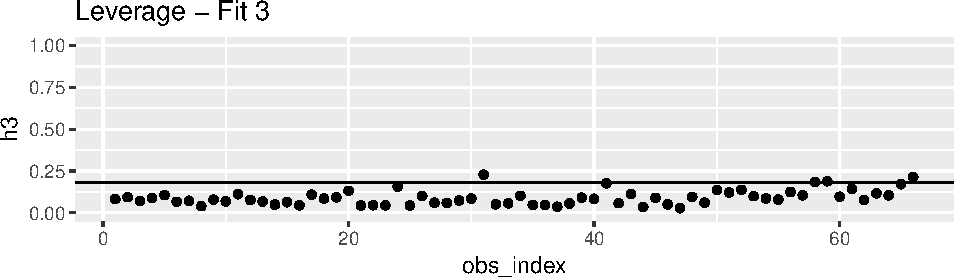
\includegraphics{20190422_multicollinearity_files/figure-latex/unnamed-chunk-20-1.pdf}

\begin{Shaded}
\begin{Highlighting}[]
\KeywordTok{ggplot}\NormalTok{(}\DataTypeTok{data =}\NormalTok{ census_transformed, }\DataTypeTok{mapping =} \KeywordTok{aes}\NormalTok{(}\DataTypeTok{x =}\NormalTok{ obs_index, }\DataTypeTok{y =}\NormalTok{ studres3)) }\OperatorTok{+}
\StringTok{  }\KeywordTok{geom_point}\NormalTok{() }\OperatorTok{+}
\StringTok{  }\KeywordTok{ggtitle}\NormalTok{(}\StringTok{"Studentized Residuals - Fit 3"}\NormalTok{)}
\end{Highlighting}
\end{Shaded}

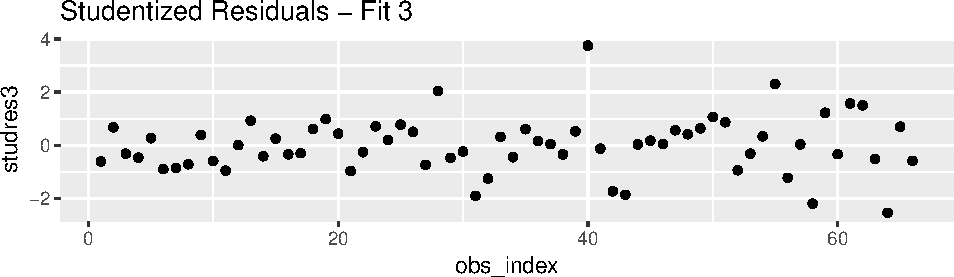
\includegraphics{20190422_multicollinearity_files/figure-latex/unnamed-chunk-20-2.pdf}

\begin{Shaded}
\begin{Highlighting}[]
\KeywordTok{ggplot}\NormalTok{(}\DataTypeTok{data =}\NormalTok{ census_transformed, }\DataTypeTok{mapping =} \KeywordTok{aes}\NormalTok{(}\DataTypeTok{x =}\NormalTok{ obs_index, }\DataTypeTok{y =}\NormalTok{ D3)) }\OperatorTok{+}
\StringTok{  }\KeywordTok{geom_point}\NormalTok{() }\OperatorTok{+}
\StringTok{  }\KeywordTok{ggtitle}\NormalTok{(}\StringTok{"Cook's Distance - Fit 3"}\NormalTok{)}
\end{Highlighting}
\end{Shaded}

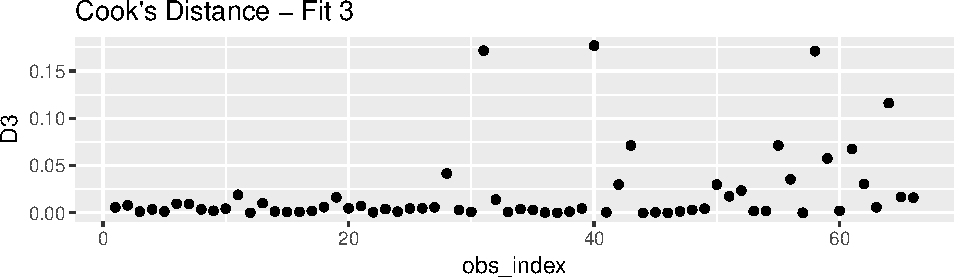
\includegraphics{20190422_multicollinearity_files/figure-latex/unnamed-chunk-20-3.pdf}

Yes. Are our findings robust to whether or not these observations are
included?

\begin{Shaded}
\begin{Highlighting}[]
\NormalTok{suspicious_obs <-}\StringTok{ }\KeywordTok{c}\NormalTok{(}\DecValTok{31}\NormalTok{, }\DecValTok{40}\NormalTok{, }\DecValTok{58}\NormalTok{, }\DecValTok{66}\NormalTok{)}
\NormalTok{census_transformed_nosuspicious <-}\StringTok{ }\NormalTok{census_transformed[}\OperatorTok{-}\NormalTok{suspicious_obs, ]}

\NormalTok{fit3_nosuspicious <-}\StringTok{ }\KeywordTok{lm}\NormalTok{(}
\NormalTok{  undercount }\OperatorTok{~}\StringTok{ }\NormalTok{minority }\OperatorTok{+}\StringTok{ }\NormalTok{poverty }\OperatorTok{+}\StringTok{ }\NormalTok{language }\OperatorTok{+}\StringTok{ }\NormalTok{geographic_unit }\OperatorTok{+}\StringTok{ }\NormalTok{conventional,}
  \DataTypeTok{data =}\NormalTok{ census_transformed_nosuspicious)}

\KeywordTok{summary}\NormalTok{(fit3_nosuspicious)}
\end{Highlighting}
\end{Shaded}

\begin{verbatim}
## 
## Call:
## lm(formula = undercount ~ minority + poverty + language + geographic_unit + 
##     conventional, data = census_transformed_nosuspicious)
## 
## Residuals:
##     Min      1Q  Median      3Q     Max 
## -3.7371 -0.6246 -0.0500  0.7937  2.7357 
## 
## Coefficients:
##                      Estimate Std. Error t value Pr(>|t|)    
## (Intercept)           3.82448    1.74793   2.188 0.032858 *  
## minority              0.28256    0.05733   4.929 7.73e-06 ***
## poverty              -0.99338    0.41873  -2.372 0.021135 *  
## language              0.41730    0.29447   1.417 0.161987    
## geographic_unitstate -2.47668    0.65065  -3.806 0.000352 ***
## conventional          0.64648    0.11973   5.400 1.41e-06 ***
## ---
## Signif. codes:  0 '***' 0.001 '**' 0.01 '*' 0.05 '.' 0.1 ' ' 1
## 
## Residual standard error: 1.248 on 56 degrees of freedom
## Multiple R-squared:  0.7567, Adjusted R-squared:  0.735 
## F-statistic: 34.84 on 5 and 56 DF,  p-value: 5.153e-16
\end{verbatim}

\begin{Shaded}
\begin{Highlighting}[]
\KeywordTok{confint}\NormalTok{(fit3_nosuspicious)}
\end{Highlighting}
\end{Shaded}

\begin{verbatim}
##                           2.5 %     97.5 %
## (Intercept)           0.3229632  7.3259979
## minority              0.1677125  0.3974114
## poverty              -1.8322023 -0.1545590
## language             -0.1725940  1.0071887
## geographic_unitstate -3.7800868 -1.1732740
## conventional          0.4066323  0.8863249
\end{verbatim}

How about residuals diagnostics for linearity/normality/etc?

\begin{Shaded}
\begin{Highlighting}[]
\NormalTok{census_transformed <-}\StringTok{ }\NormalTok{census_transformed }\OperatorTok
\StringTok{  }\KeywordTok{mutate}\NormalTok{(}
    \DataTypeTok{residual =} \KeywordTok{residuals}\NormalTok{(fit3),}
    \DataTypeTok{suspicious =} \KeywordTok{row_number}\NormalTok{() }\OperatorTok\StringTok{ }\NormalTok{suspicious_obs}
\NormalTok{  )}

\KeywordTok{ggplot}\NormalTok{(}\DataTypeTok{data =}\NormalTok{ census_transformed, }\DataTypeTok{mapping =} \KeywordTok{aes}\NormalTok{(}\DataTypeTok{x =}\NormalTok{ minority, }\DataTypeTok{y =}\NormalTok{ residual, }\DataTypeTok{color =}\NormalTok{ suspicious)) }\OperatorTok{+}
\StringTok{  }\KeywordTok{geom_point}\NormalTok{()}
\end{Highlighting}
\end{Shaded}

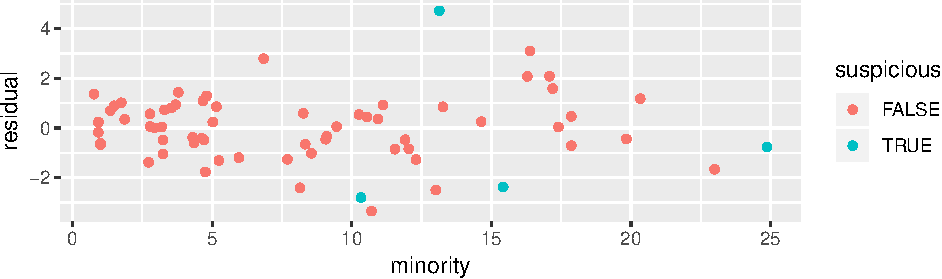
\includegraphics{20190422_multicollinearity_files/figure-latex/unnamed-chunk-22-1.pdf}

\begin{Shaded}
\begin{Highlighting}[]
\KeywordTok{ggplot}\NormalTok{(}\DataTypeTok{data =}\NormalTok{ census_transformed, }\DataTypeTok{mapping =} \KeywordTok{aes}\NormalTok{(}\DataTypeTok{x =}\NormalTok{ poverty, }\DataTypeTok{y =}\NormalTok{ residual, }\DataTypeTok{color =}\NormalTok{ suspicious)) }\OperatorTok{+}
\StringTok{  }\KeywordTok{geom_point}\NormalTok{()}
\end{Highlighting}
\end{Shaded}

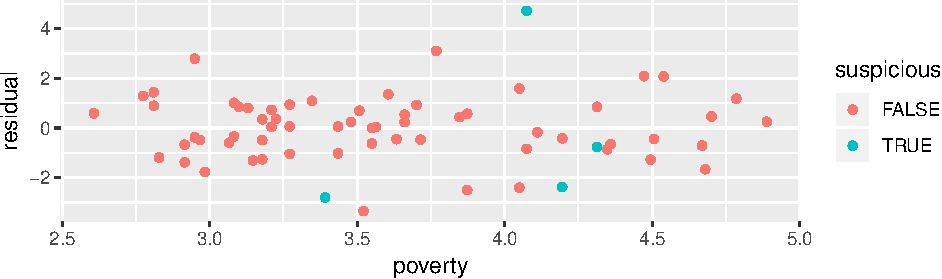
\includegraphics{20190422_multicollinearity_files/figure-latex/unnamed-chunk-22-2.pdf}

\begin{Shaded}
\begin{Highlighting}[]
\KeywordTok{ggplot}\NormalTok{(}\DataTypeTok{data =}\NormalTok{ census_transformed, }\DataTypeTok{mapping =} \KeywordTok{aes}\NormalTok{(}\DataTypeTok{x =}\NormalTok{ language, }\DataTypeTok{y =}\NormalTok{ residual, }\DataTypeTok{color =}\NormalTok{ suspicious)) }\OperatorTok{+}
\StringTok{  }\KeywordTok{geom_point}\NormalTok{()}
\end{Highlighting}
\end{Shaded}

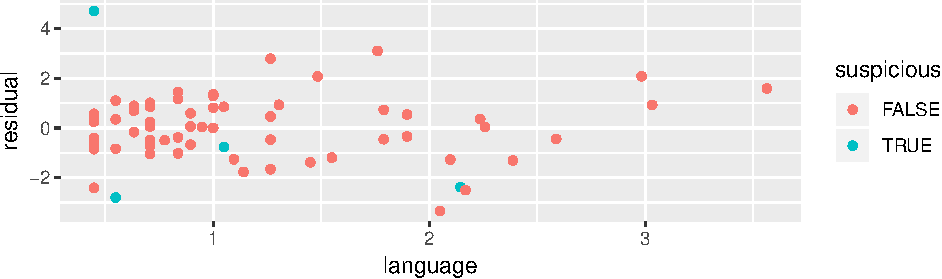
\includegraphics{20190422_multicollinearity_files/figure-latex/unnamed-chunk-22-3.pdf}

\begin{Shaded}
\begin{Highlighting}[]
\KeywordTok{ggplot}\NormalTok{(}\DataTypeTok{data =}\NormalTok{ census_transformed, }\DataTypeTok{mapping =} \KeywordTok{aes}\NormalTok{(}\DataTypeTok{x =}\NormalTok{ residual, }\DataTypeTok{color =}\NormalTok{ geographic_unit, }\DataTypeTok{color =}\NormalTok{ suspicious)) }\OperatorTok{+}
\StringTok{  }\KeywordTok{geom_density}\NormalTok{()}
\end{Highlighting}
\end{Shaded}

\begin{verbatim}
## Warning: Duplicated aesthetics after name standardisation: colour
\end{verbatim}

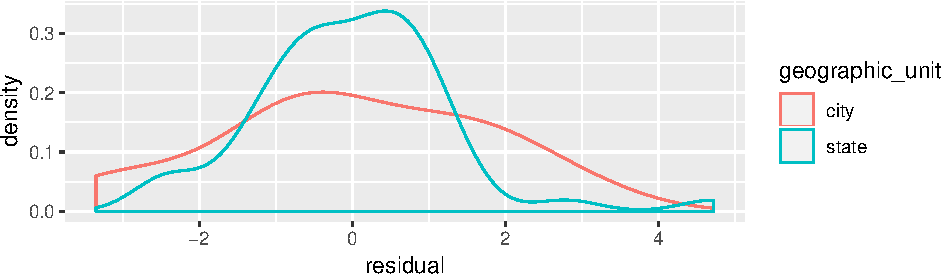
\includegraphics{20190422_multicollinearity_files/figure-latex/unnamed-chunk-22-4.pdf}

\begin{Shaded}
\begin{Highlighting}[]
\NormalTok{census_transformed }\OperatorTok
\StringTok{  }\KeywordTok{group_by}\NormalTok{(geographic_unit) }\OperatorTok
\StringTok{  }\KeywordTok{summarize}\NormalTok{(}\KeywordTok{sd}\NormalTok{(residual))}
\end{Highlighting}
\end{Shaded}

\begin{verbatim}
## # A tibble: 2 x 2
##   geographic_unit `sd(residual)`
##   <fct>                    <dbl>
## 1 city                      1.79
## 2 state                     1.26
\end{verbatim}

\begin{Shaded}
\begin{Highlighting}[]
\KeywordTok{ggplot}\NormalTok{(}\DataTypeTok{data =}\NormalTok{ census_transformed, }\DataTypeTok{mapping =} \KeywordTok{aes}\NormalTok{(}\DataTypeTok{x =}\NormalTok{ conventional, }\DataTypeTok{y =}\NormalTok{ residual, }\DataTypeTok{color =}\NormalTok{ suspicious)) }\OperatorTok{+}
\StringTok{  }\KeywordTok{geom_point}\NormalTok{()}
\end{Highlighting}
\end{Shaded}

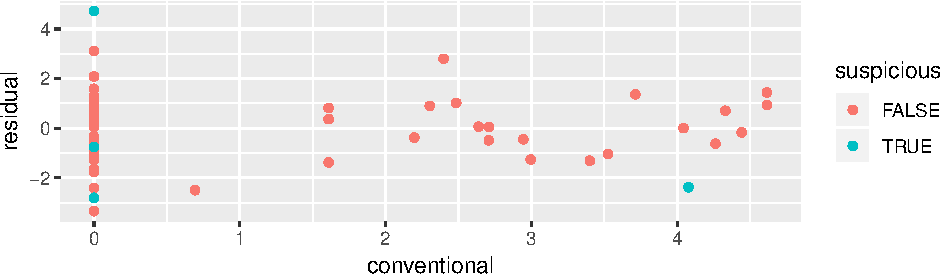
\includegraphics{20190422_multicollinearity_files/figure-latex/unnamed-chunk-22-5.pdf}

\newpage

\paragraph{What are our conclusions?}\label{what-are-our-conclusions}

\begin{itemize}
\tightlist
\item
  We found consistent and strong evidence that higher concentrations of
  minorities and higher rates of use of conventional census methods were
  both associated with larger census undercounts, after controlling for
  the other covariates selected for inclusion in the model.
\item
  We also found consistent and strong evidence that census undercounts
  were larger in large cities than in the other parts of those states or
  other states taken as a whole, after accounting for the associations
  of other covariates with census undercounts.
\item
  These findings were robust to the covariates included in our model,
  and held whether or not four outlying high leverage observations were
  included.
\item
  We saw less consistent associations between census undercounts and the
  poverty rate, crime rate, and rate at which residents had difficulty
  speaking or writing in English, after controlling for the associations
  found above. These variables were not always included in models
  selected by BIC, and the strength of evidence of an association with
  the census undercount depended on which other covariates were included
  and whether or not high leverage observations were included.
\item
  This is an observational study and our findings are limited in scope
  to the particular regions included in the analysis, and to the
  procedures used 1980 Census.
\end{itemize}

\paragraph{In the authors' words\ldots{}}\label{in-the-authors-words}

\begin{itemize}
\tightlist
\item
  Here's what they said about their variable selection procedure
\end{itemize}

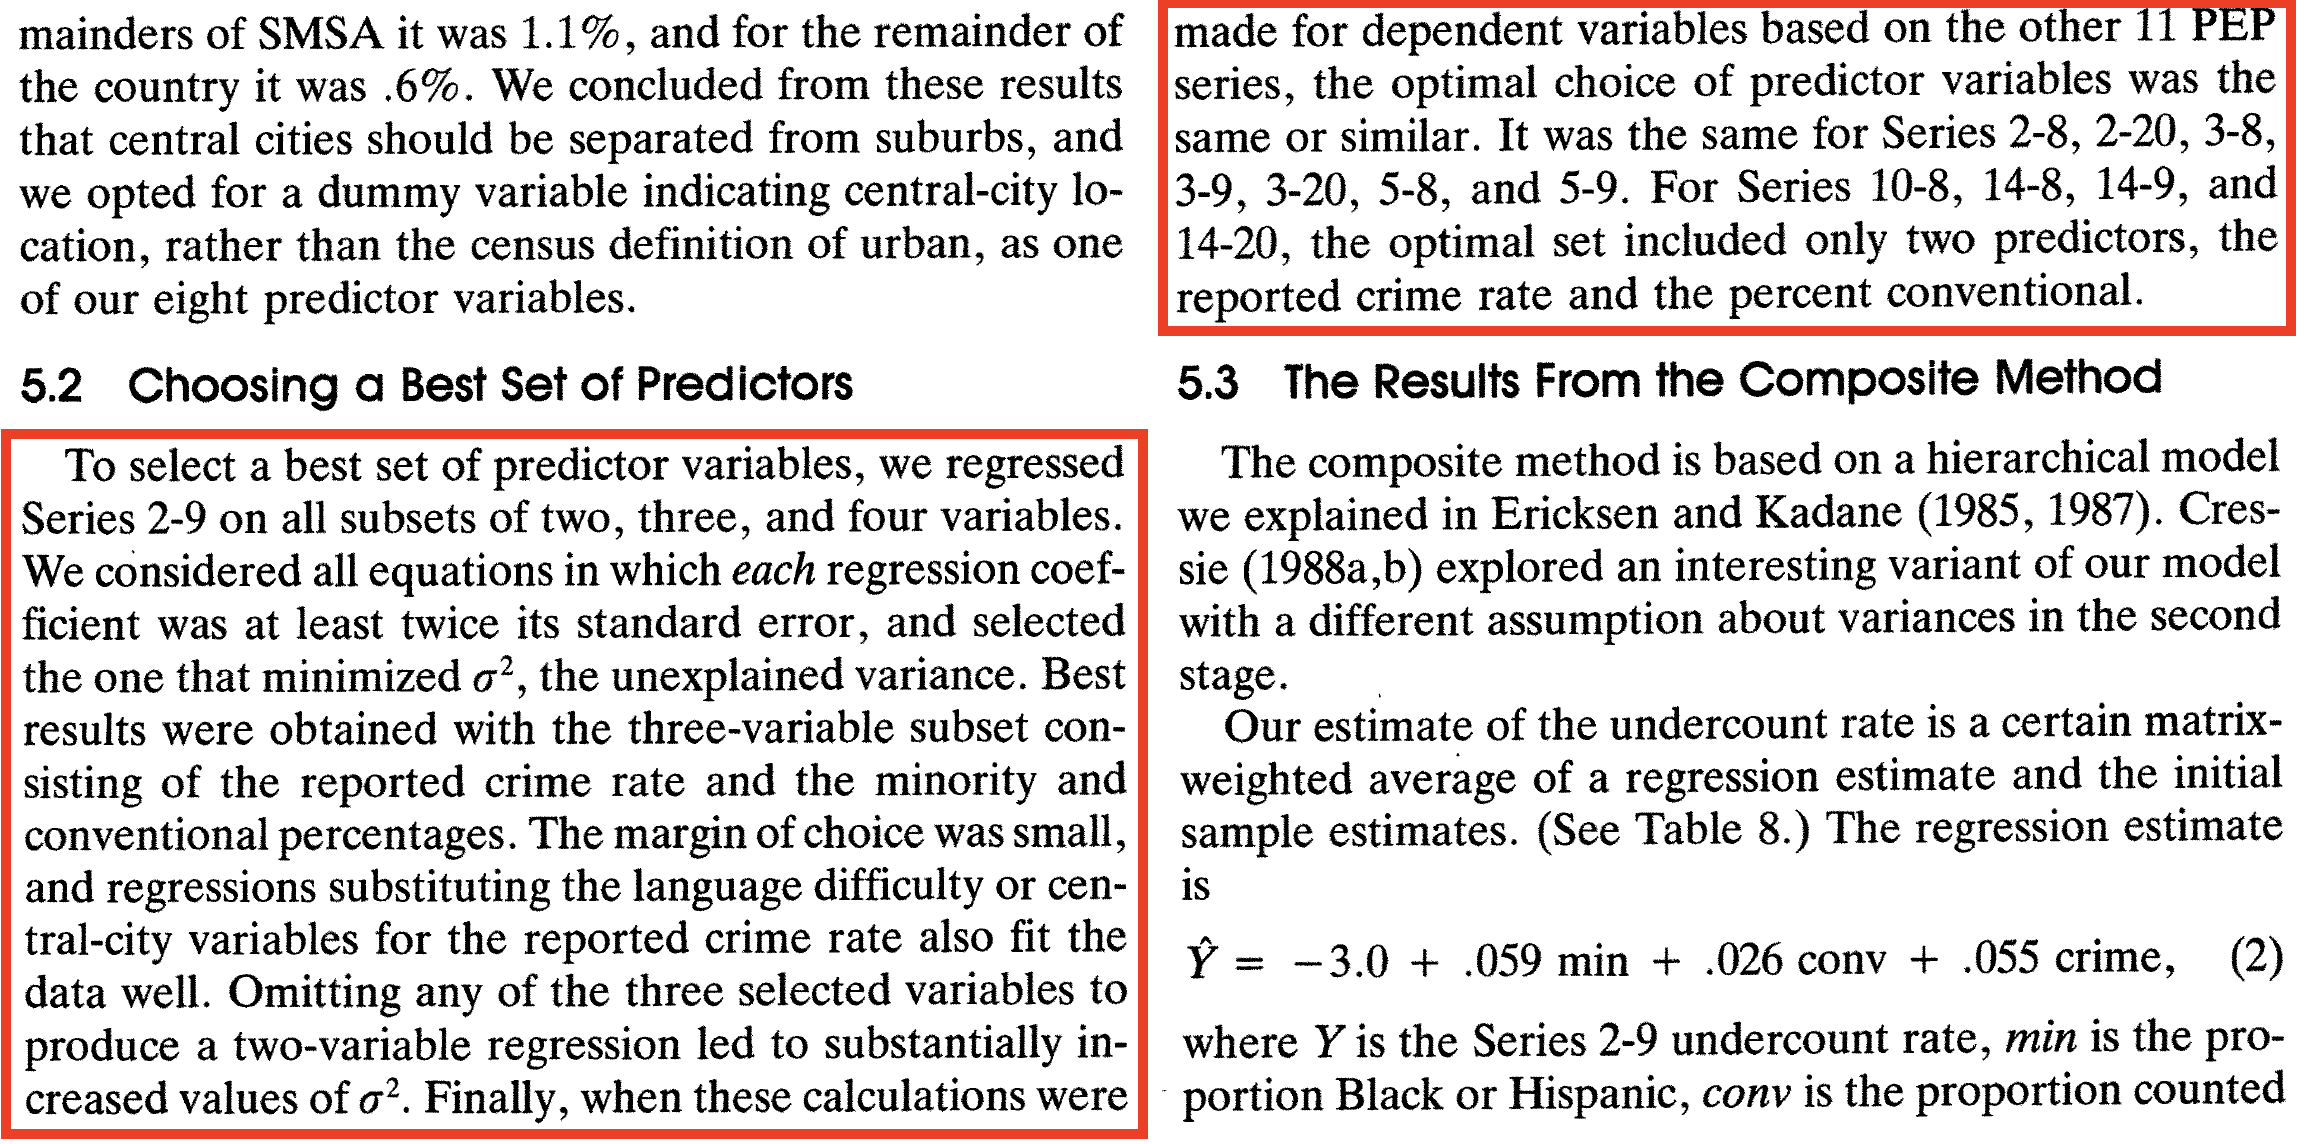
\includegraphics[width=8in]{Ericksen_var_selection.png}

\begin{itemize}
\tightlist
\item
  Here is the first paragraph of the conclusions:
\end{itemize}

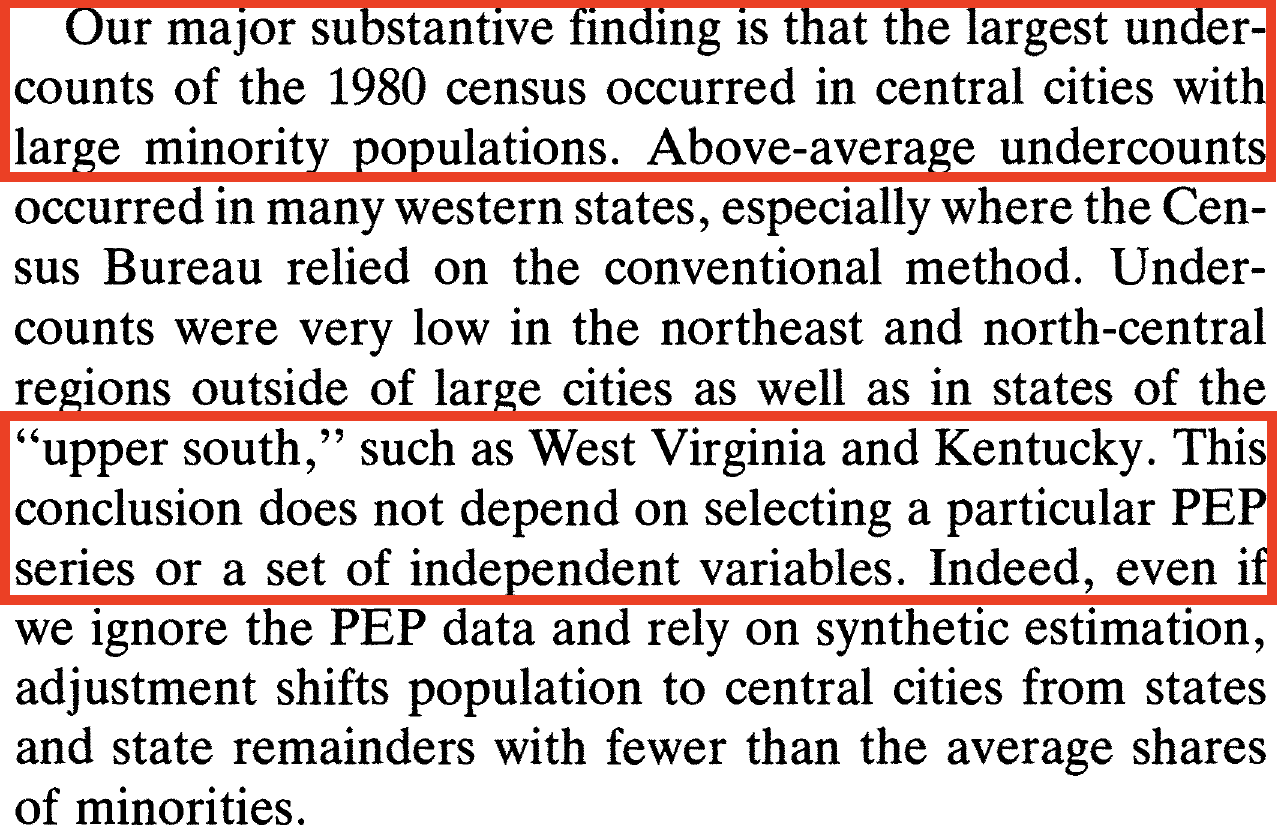
\includegraphics[width=4in]{Ericksen_conclusions.png}

\begin{itemize}
\tightlist
\item
  Here is a statement of the scope of conclusions, second paragraph of
  conclusions:
\end{itemize}

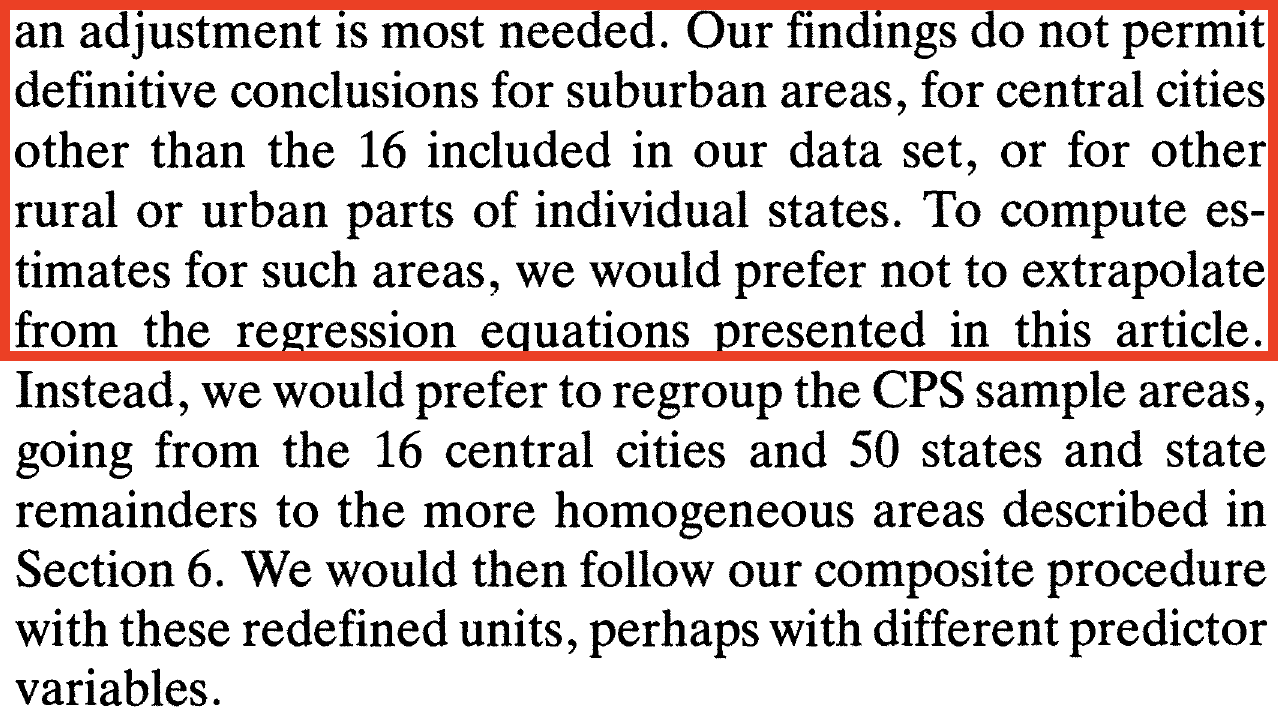
\includegraphics[width=4in]{Ericksen_scope.png}


\end{document}
